\documentclass[11pt]{article}
\usepackage{amsmath, amssymb, amsthm}
\usepackage[retainorgcmds]{IEEEtrantools}

\usepackage[pdftex]{graphicx}
\usepackage{tikz}
\usetikzlibrary{intersections}

\usepackage{marginnote}
\usepackage{endnotes}

\usepackage{fancyhdr}

%Listings stuff
\usepackage{listings}
\usepackage{lstautogobble}
\usepackage{color}

\definecolor{gray}{rgb}{0.5,0.5,0.5}
\lstset{
basicstyle={\small\ttfamily},
tabsize=3,
numbers=left,
numbersep=5pt,
numberstyle=\tiny\color{gray},
stepnumber=2,
breaklines=true
}

%Properly formatted differential 'd'
\newcommand{\ud}{\, \mathrm{d}}

%Format stuff
\pagestyle{fancy}
\headheight 35pt

%Header info
\chead{\Large \textbf{Equations and Matrices}}
\lhead{}
\rhead{}

\begin{document}
\section{Gaussian Elimination}
	Given a linear system of equations represented by $\mathbf{A}\vec{x} = \vec{b}$, where the matrix $\mathbf{A}$ represents the coefficients of the unknowns or variables in $\vec{x}$, it is possible with a series of basic manipulations to come up with a solution.
	
	\begin{equation}
		\left(\begin{matrix}
			a & b & c & | & d\\
			e & f & g & | & h\\
			i & j & k & | & l
		\end{matrix}\right)
	\end{equation}
	
	Turn $a$ into 1, and then use the top equation to zero out $e$ and $i$ by combining the rows with a scalar multiple of the first row.
	
	\begin{equation}
		\left(\begin{matrix}
			1 & m & n & | & o\\
			0 & p & q & | & r\\
			0 & s & t & | & u
		\end{matrix}\right)
	\end{equation}
	
	Turn $p$ into 1, and then turn $s$ into 0 by using the same method. Back substitute to obtain either an unique answer, a line, or an empty set of solutions.
	
	\begin{equation}
		\left(\begin{matrix}
			1 & m & n & | & o\\
			0 & 1 & v & | & w\\
			0 & 0 & x & | & y
		\end{matrix}\right)
	\end{equation}
	
	\subsection{Geometric Representation}
		In $\mathbb{R}^3$, the system of equations can be thought of as solving for the intersection of 3 planes - see Figure \ref{fig:planarint}. The solution can either be a single point, a line, or nothing. If one equation reduces to $0 = 0$ or some other tautology, then assign one variable (usually $z$) to be a \textbf{free variable} - the parameter - by turning it into $t$, and adding a third equation $z = t$. Then it is possible to express the system like such.
		\begin{IEEEeqnarray}{rCl}
			x & = & k_1t + c_1\\
			y & = & k_2t + c_2\\
			z & = & t
		\end{IEEEeqnarray}
		
	\begin{figure}[htb]
		\centering
		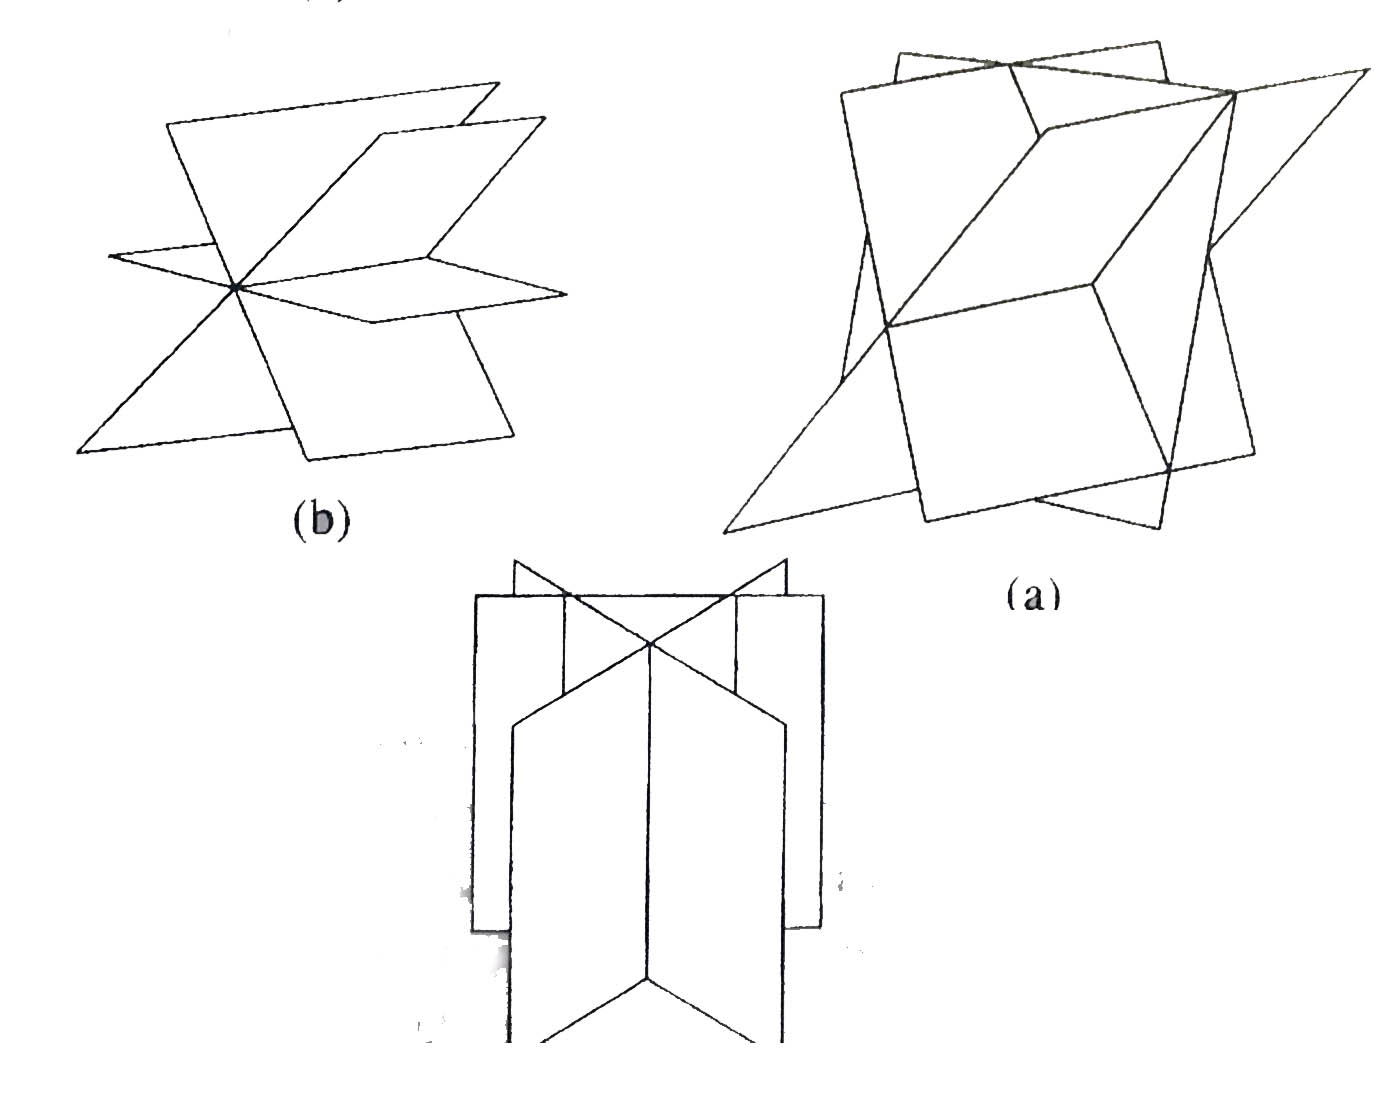
\includegraphics[width=0.5\textwidth]{planarint.jpg}
		\caption{Three cases of planes intersecting.}
		\label{fig:planarint}
	\end{figure}
	
\section{Matrix Algebra}
	Matrix addition and subtraction works exactly like you think it does, as long as both matrices have equal dimensions. Scalar multiplication works the same way as well. The \textbf{zero matrix} is notated as $O$, and has the property $A + O = A$.
	
	\subsection{Matrix Multiplication}
		If $A$ is $m-\text{by}-n$ and $b$ is $n-\text{by}-p$, the matrix product $AB$ is the $m-\text{by}-p$ matrix $C$ where $c_{ij}$ is the dot product of the $i$\textsuperscript{th} row of $A$ and the $j$\textsuperscript{th} column of $B$. In summation notation, where $k$ runs over the column index of $A$ and the row index of $B$:
		\begin{equation}
			AB_{ij} = \sum_{k=1}^n a_{ik}b_{kj}
		\end{equation}
		
		Note that matrix multiplication is not in general commutative. There are 4 basic properties of matrix multiplication, listed below.
		\begin{center}
			\begin{tabular}{r|l}
				Law							& Example\\\hline
				Right distributive			& $(A+B)C = AC+BC$\\
				Left distributive			& $C(A+B) = CA+CB$\\
				Scalar commutativity		& $(tA)B=t(AB)=A(tB)$\\
				Associative					& $A(BC)=(AB)C$
			\end{tabular}
		\end{center}
		
		\subsection{Identity Matrix}
			An identity matrix is a square matrix with 1s on its \textbf{main diagonal} and 0s elsewhere, and has the following property.
			\begin{equation}
				IA=AI=A
			\end{equation}
			
		\subsection{Matrix Polynomials}
			If $A$ is a square matrix, then we can raise $A$ to powers, where $A^0$ is the identity matrix.
			
\section{Inverse Matrices}
	If $A$ and $B$ are square matrices with equal dimensions and $AB = I$, then $B$ is an \textbf{inverse} of $A$ and $A$ is an \textbf{invertible} matrix.
	\begin{equation}
		AA^{-1} = A^{-1}A = I
	\end{equation}
	If $A$ is invertible, then the system of equations $A\vec{x}=b$ has a unique solution $\vec{x}=A^{-1}b$. In particular, $\vec{x}=\vec{0}$ is the only solution to $A\vec{x}=\vec{0}$.
	
	For a 2-by-2 matrix, it is invertible if its \textbf{determinant} $ad-bc$ is not zero.
	\begin{equation}
		\left(\begin{matrix}
			a&b\\c&d
		\end{matrix}\right)^{-1} = \frac{1}{ad-bc}\left(\begin{matrix}
			d&-b\\-c&a
		\end{matrix}\right)
	\end{equation}
	
	For larger matrices, use basic row operations and \textbf{row rearrangement} to transform the matrix $A$ into the identity matrix $I$, while performing the exact same sequence of steps on $I$ to get $A^{-1}$.
	
	\textbf{Diagonal matrices} and \textbf{upper triangular matrices} are invertible only if there are no zeroes on the main diagonal. In the latter case, it is easier to reduce the columns working from right to left.
	\begin{equation}
		\begin{pmatrix}
			b_1 & 0 & 0\\
			0 & b_2 & 0\\
			0 & 0 & b_3
		\end{pmatrix}
	\end{equation}
	\begin{equation}
		\begin{pmatrix}
			b_11 & b_12 & b_13\\
			0 & b_22 & b_23\\
			0 & 0 & b_33
		\end{pmatrix}
	\end{equation}
%	\begin{center}
%	\begin{tikzpicture}
%		[scale=3,line cap=round,
%		%Styles
%		axes/.style=,
%		important line/.style={very thick},
%		information text/.style={rounded corners,fill=red!10,inner sep=1ex},
%		dot/.style={circle,inner sep=1pt,fill,label={#1},name=#1}			
%		]
%		
%		%Colors
%		\colorlet{anglecolor}{green!50!black}	%angle arcs/lines
%		
%		%The graphic
%	\end{tikzpicture}
%	\end{center}

%	\begin{figure}[htb]
%		\centering
%		\includegraphics[width=0.8\textwidth]{filename.eps}
%		\caption{Caption.}
%		\label{fig:figure}
%	\end{figure}

%		\def\enotesize{\normalsize}
%		\theendnotes
\end{document}